
\documentclass[a4paper]{report}
% \documentclass{report}
\usepackage[utf8]{inputenc}
\usepackage{amsmath}
\usepackage{esint}
\usepackage{tabstackengine}
\usepackage[colorlinks,linkcolor=blue]{hyperref}
\usepackage{xeCJK}
\usepackage{caption}
\usepackage{stackengine}
\usepackage{graphicx}
\graphicspath{ {../resources/figure/microwave/} }
\usepackage{float}
\usepackage{amsmath}
\usepackage{ulem}
\usepackage{amsfonts}
\usepackage{blkarray}
\usepackage{enumitem}
\setlist[1]{itemsep=-5pt}
\usepackage{subcaption}

\usepackage{tikz}
\usetikzlibrary{calc}
\usepackage{pgfplots}
\usepackage{mathrsfs}
\usetikzlibrary{shapes,arrows,positioning}
\captionsetup[table]{skip=10pt}

%%%% 下面的命令重定义页面边距,使其符合中文刊物习惯 %%%%
\addtolength{\topmargin}{-54pt}
\setlength{\oddsidemargin}{0.63cm}  % 3.17cm - 1 inch
\setlength{\evensidemargin}{\oddsidemargin}
\setlength{\textwidth}{14.66cm}
\setlength{\textheight}{24.00cm}    % 24.62


% 段首不缩进
\setlength{\parindent}{0pt}
%%%% 下面的命令设置行间距与段落间距 %%%%
\linespread{1.2}
% \setlength{\parskip}{1ex}
\setlength{\parskip}{.5\baselineskip}

\def\rlwd{.5pt} \def\rlht{2.2ex} \def\rldp{.5ex}
\def\mydiv#1{~%
  \rule[-\rldp]{\rlwd}{\rlht}%
  \setbox0=\hbox{~#1}%
  \stackunder[\dimexpr\rldp-\rlwd]{~#1}{\rule{\wd0}{\rlwd}}%
}

\title{Microwave}
\author{Crosstyan}
\date{Dec 2020}


\begin{document}
\chapter{Electromagnetic Theory}
300MHz$\sim$3000GHz$\Leftrightarrow$1m$\sim$1mm. 
$$f\cdot \lambda=c$$
\section{Maxwell Equation}
\begin{align*}
   \nabla \times \vec{H}&=\frac{\partial \vec{D}}{\partial t}+\vec{J}
 \\ \nabla \times \vec{E}&=-\frac{\partial \vec{B}}{\partial t}
  \\ \nabla \cdot \vec{B}&=0
  \\ \nabla \cdot \vec{D}&=\rho
\end{align*}
\section{媒质本构关系}
\begin{align*}
  \vec{D}&=\epsilon\cdot \vec{E}
  \\ \vec{B}&=\mu\cdot\vec{H}
  \\ \vec{J}&=\sigma\cdot \vec{E}
\end{align*}
\section{Boundary Condition}
\paragraph{电场强度}
\begin{align*}
  \hat{n}\times (\vec{H_1}-\vec{H_2})=\vec{J_s}
\end{align*}
叉乘为切向\\
磁场强度的切向分量是不连续的, 除非没有表面电流的存在
\paragraph{磁场强度}
\begin{align*}
  \hat{n}\times (\vec{E_1}-\vec{E_2})=0
\end{align*}
叉乘为切向\\
电场强度的切向分量是连续的
\paragraph{磁感应强度}
\begin{align*}
  \hat{n}\cdot (\vec{B_1}-\vec{B_2})=0
\end{align*}
点乘为法向\\
磁感应强度的法向分量是连续的

\paragraph{电位移矢量}
\begin{align*}
  \hat{n}\cdot (\vec{D_1}-\vec{D_2})=\rho_s
\end{align*}
点乘为法向\\
电位移矢量的法向分量是不连续的, 除非没有表面电荷的存在
\subsection{理想电介质}
\begin{align*}
  \rho_s&=0
  \\ J_s&=0
\end{align*}
右边全是0, 全都连续. 

\section{Poynting's theorem}
坡印廷定理
\section{Duality}
广义电磁场方程有
\begin{align*}
  \vec{E}=\vec{E_e}+\vec{E_m}
  \\ \vec{H}=\vec{H_e}+\vec{H_m}
\end{align*}
$\vec{E_e}$和$\vec{H_e}$是由$\vec{J_e}$和$\rho_e$产生的场
\begin{align*}
  \nabla \times \vec{E_e}&=-j\omega\mu\vec{H_e}
  \\ \nabla \times \vec{H_e}&=j\omega\epsilon\vec{E_e}+\vec{J_e}
  \\ \nabla \cdot (\mu\vec{H_e})&=0
  \\ \nabla \cdot (\epsilon\vec{E_e})&=\rho_e
\end{align*}
$\vec{E_m}$和$\vec{H_m}$是由$\vec{J_m}$和$\rho_m$产生的场
\begin{align*}
  \nabla \times \vec{E_m}&=-j\omega\mu\vec{H_m}-\vec{J_m}
  \\ \nabla \times \vec{H_m}&=j\omega\epsilon\vec{E_m}
  \\ \nabla \cdot (\mu\vec{H_m})&=0
  \\ \nabla \cdot (\epsilon\vec{E_m})&=-\rho_m
\end{align*}
对于电场引发($e$)$\Leftrightarrow$磁场引发($m$)有如下对偶变换\footnote{共十对, 左为源($e$), 右为对偶($m$)}
\begin{align*}
  \vec{E_e}\rightarrow\vec{H_m}& \quad \vec{H_e}\rightarrow -\vec{E_m}
  \\ \vec{E_m}\rightarrow\vec{H_e}&\quad\vec{H_m}\rightarrow -\vec{E_e}
  \\ \vec{J_e}\rightarrow\vec{J_m}&\quad\vec{J_m}\rightarrow -\vec{J_e}
  \\ \rho_e\rightarrow\rho_m&\quad\rho_m\rightarrow -\rho_e
  \\ \epsilon\rightarrow\mu&\quad\mu\rightarrow -\epsilon
\end{align*}
\chapter{Transmission Line Theory}
\section{Telegram Equations}
per-unit-length quantities
\begin{itemize}
  \item R: $\Omega$/m
  \item L: H/m
  \item G: S/m
  \item C: F/m
\end{itemize}
Differential equations
\begin{align*}
  \frac{\partial v(z,t) }{\partial z}=-R\cdot i(z,t)-L\cdot \frac{\partial i(z,t) }{\partial z}
  \\ \frac{\partial i(z,t) }{\partial z}=-G\cdot i(z,t)-C\cdot \frac{\partial v(z,t) }{\partial z}
\end{align*}

with phasors, simplify to
\begin{align*}
  \frac{d V(z)}{dz}=-(R+j\omega L)\cdot I(z)
  \\ \frac{d I(z)}{dz}=-(G+j\omega C)\cdot V(z)
\end{align*}
with propagation constant
\begin{align*}
  \gamma= \alpha+j\beta=\sqrt{(R+j\omega L)\cdot (G+j\omega C)}
\end{align*}
simplify to 
\begin{align*}
  \frac{d^2 V(z)}{dz^2}-\gamma^2\cdot V(z)=0
  \\ \frac{d^2 I(z)}{dz^2}-\gamma^2\cdot I(z)=0
\end{align*}
\section{Lossless Line}
propagation constant $\gamma$
\begin{align*}
  \gamma=\alpha+j\beta
  \\ \beta=\omega\cdot\sqrt{LC}
  \\ \alpha=0
\end{align*}
The characteristic impedance 
\begin{align*}
  Z_0=\sqrt{\frac{L}{C}}
\end{align*}
The general solutions for voltage and current on a lossless transmission line
\begin{align}
  V(z)=V_0^+\cdot e^{-j\beta z}+V_0^-\cdot e^{j\beta z}
  \\I(z)=\frac{V_0^+}{Z_0}\cdot e^{-j\beta z}-\frac{V_0^-}{Z_0}\cdot e^{j\beta z}
  \label{eq:general_solution}
\end{align}
$V_0^+,V_0^-,I_0^+,I_0^-$是待定系数, 右上角的$+,-$与指数前的符号相反\footnote{若以右为$z$轴正方向则相反, 若以左为$z$轴正方向则一致. 在此$+$代表入射波, $-$代表反射波}

The wavelength is
\begin{align*}
  \lambda=\frac{2\pi}{\beta}=\frac{2\pi}{\omega\sqrt{LC}}
\end{align*}
The phase velocity is 
\begin{align*}
  v_p=\frac{\omega}{\beta}=\frac{1}{\sqrt{LC}}
\end{align*}
\section{Terminated Lossless Transmission Line}
General solution
\begin{align*}
  V(z)=V_0^+\cdot e^{-j\beta z}+V_0^-\cdot e^{j\beta z}
  \\I(z)=\frac{V_0^+}{Z_0}\cdot e^{-j\beta z}-\frac{V_0^-}{Z_0}\cdot e^{j\beta z}
\end{align*}
\begin{figure}[H]
\centering
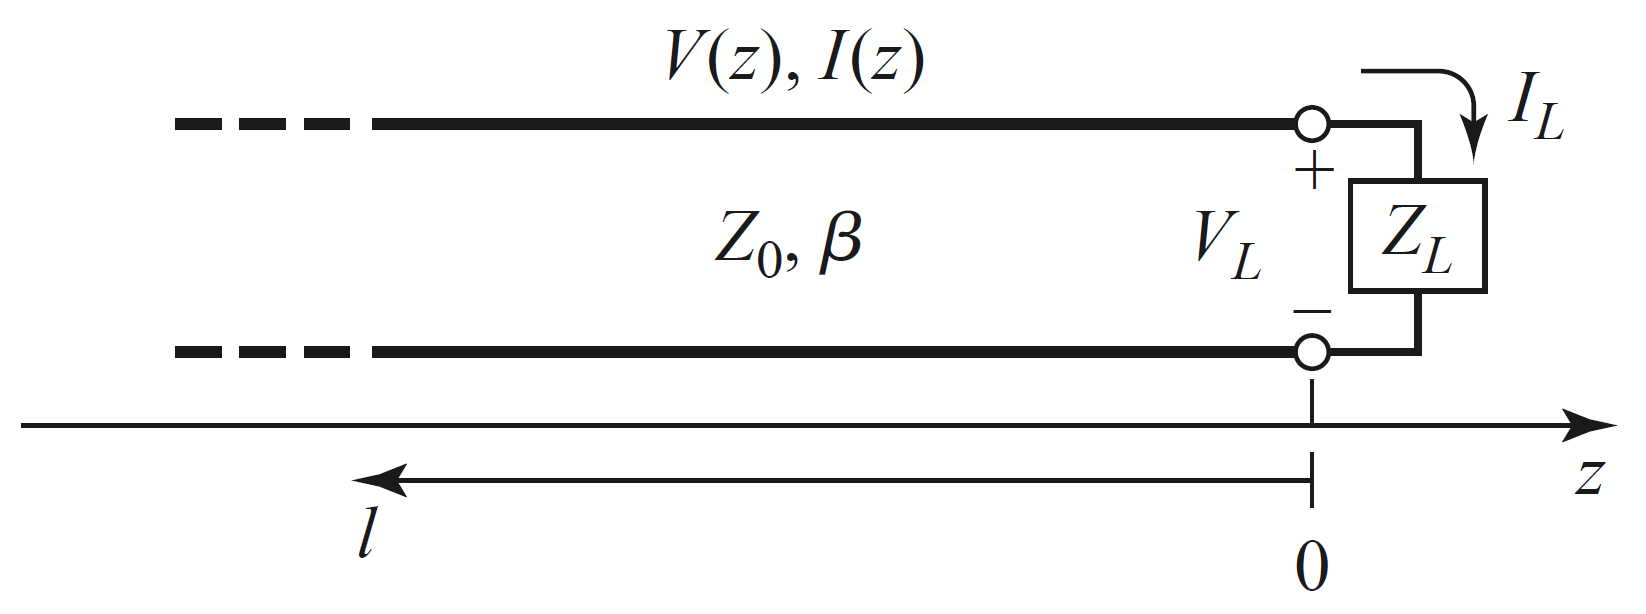
\includegraphics[width=0.7\textwidth]{tl.png}
\caption{A transmission line terminated in a load impedance $Z_L$}
\end{figure}
Load impedance\footnote{$Z(0)$位于终端, 即以终端为原点, $z$轴坐标轴方向与入射波传播方向一致(与微波工程基础中定义的传播方向不同)} 
\begin{align*}
  Z_L=\frac{V(0)}{I(0)}=\frac{V_0^+ + V_0^-}{I_0^+ - I_0^-}
\end{align*}
$Z_L$为负载阻抗, $Z_0$为本征阻抗(特征阻抗)

Solving for $V_0^-$ gives
\begin{align*}
  V_0^-=\frac{Z_L-Z_0}{Z_L+Z_0}\cdot V_0^+
\end{align*}
the coefficient\footnote{反射波等于入射波前面乘一个系数, 那个系数就是反射系数啦} is defined as the \textbf{voltage reflection coefficient}, $\Gamma$

\begin{align}
  \Gamma_L=\Gamma=\frac{Z_L-Z_0}{Z_L+Z_0}
\end{align}
在均匀传输线上时
\begin{align*}
   \Gamma(\underset{\text{distance to load}}{l})=\Gamma_L\cdot e^{j2\beta l}
\end{align*}

The general solution can be written as \footnote{再次注意, 这里是以$-z$为入射波, $+z$为反射波, 故反射系数加在$+z$前}
\begin{align}
  V(z)=V_0^+\cdot(e^{-j\beta z}+\Gamma\cdot e^{j\beta z})
  \\  I(z)=I_0^+\cdot(e^{-j\beta z}-\Gamma\cdot e^{j\beta z})
\end{align}
\textbf{Voltage Standing Wave Ratio} (VSWR) 驻波比\footnote{有的教材叫$\rho$}

$$
  \text{SWR}=\frac{V_{\max}}{V_{\min}}=
  \frac{1+\lvert \Gamma \rvert}{1-\lvert \Gamma \rvert}
$$
\subsection{Special Cases}
\subsubsection{行波状态}
后边接匹配负载
\begin{align*}
  Z_L=Z_0
\end{align*}
\begin{itemize}
  \item 沿线电压和电流振幅不变, 反射系数为0
  \item 电压和电流在任一点同相
  \item 传输线上各点阻抗均等于传输线特性阻抗
\end{itemize}
\subsubsection{纯驻波状态}
后边是短路负载或者开路负载
\subsubsection{Half-wavelength}
阻抗的周期性:输入阻抗以1/2波长为周期. 因为反射系数的周期为1/2波长. 
\begin{align*}
  Z(z)&=Z(z+\frac{\lambda}{2})
\end{align*}
在均匀传输线上时\footnote{若以$-z$为反射波方向(微博工程基础定义), 则指数部分应为负数$e^{-j2\beta l}$}
\begin{align*}
   \Gamma(\underset{\text{distance to load}}{l})=\Gamma_L\cdot e^{j2\beta l}
\end{align*}
\subsubsection{Quarter-wavelength}
归一化阻抗的倒置性指两个相距1/4波长截面处的归一化输入阻抗互为倒数。\footnote{$\bar{z}$表示归一化阻抗}
\begin{align*}
  Z(z+\frac{\lambda}{4})&=\frac{Z_0^2}{Z(z)}
  \\ \bar{z} (z+\frac{\lambda}{4})&=\frac{1}{ \bar{z} (z)}
\end{align*}
\subsubsection{Junction}
consider a transmission line of characteristic impedance $Z_0$ feeding a line of different characteristic impedance $Z_1$
\begin{figure}[H]
\centering
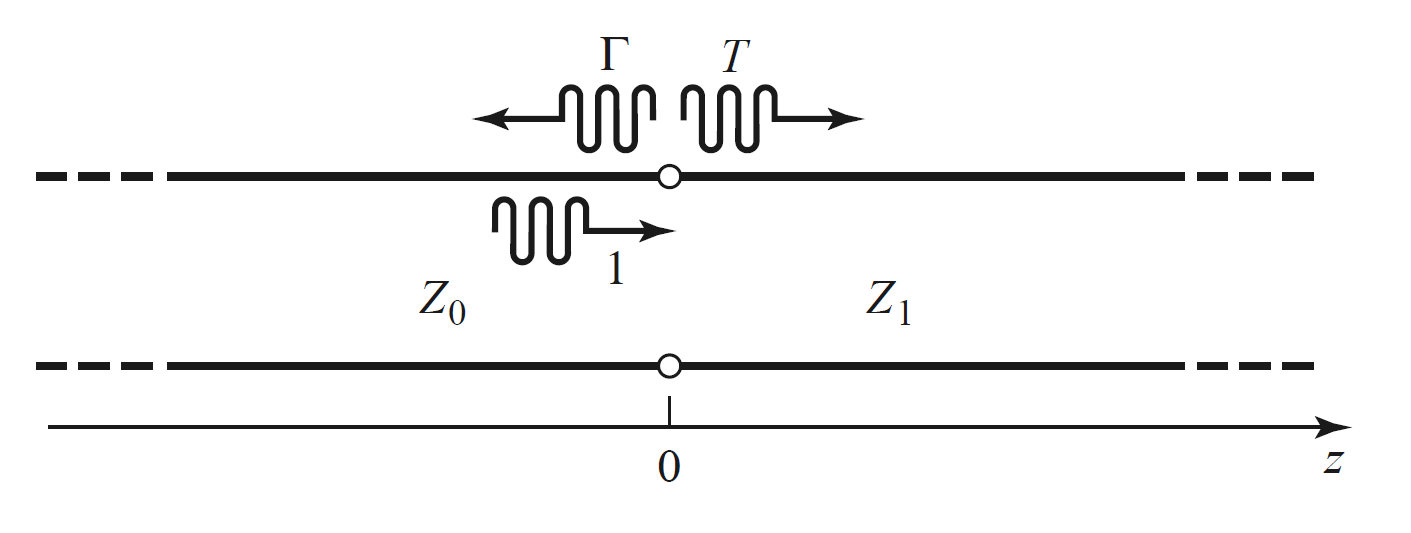
\includegraphics[width=0.7\textwidth]{junction.png}
\caption{Junction}
\end{figure}
\begin{align*}
\Gamma(\text{at junction})=\frac{Z_1-Z_0}{Z_1+Z_0}
\end{align*}
\paragraph{TRANSM. COEFF, E or I}传输系数
\begin{align*}
  T=1+\Gamma=\frac{2\cdot Z_1}{Z_1+Z_0}
\end{align*}

\section{The Smith Chart}
If a lossless line of characteristic impedance $Z_0$ is terminated a with a load impedance $Z_L$, the reflection coefficient at the load can be written as
\begin{align*}
  \Gamma&=\frac{z_L-1}{z_L+1}=\lvert \Gamma \rvert\cdot e^{j\theta}
  \\z_L&=r_L+j\cdot x_L
  \\z_L&=\frac{Z_L}{Z_0}
\end{align*}
\paragraph{SWR}驻波比 (VSWR)
\paragraph{RTN.LOSS}返回损失 (in dB)
\begin{align*}
  \text{return loss}=-20\cdot \lg{\lvert \Gamma \rvert}
\end{align*}
\paragraph{RFL. COEFF, P}功率反射系数, 就是$\Gamma^2$
\paragraph{RFL. COEFF, E or I}反射系数, 就是$\Gamma$

\section{Impedance Matching}
\subsection{Matching with lumped elements}
集总元件阻抗匹配 (不考)
\subsection{Single-stub tuning}
\begin{figure}[H]
\centering
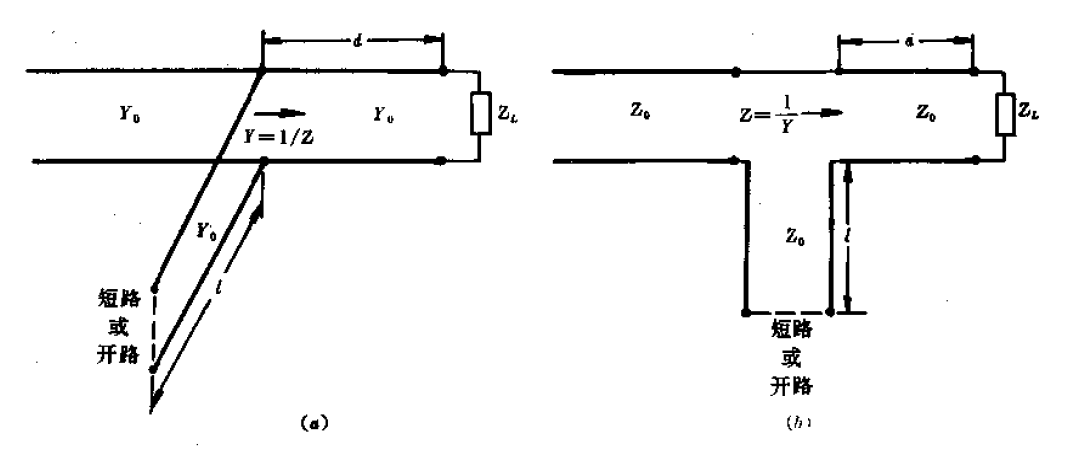
\includegraphics[width=0.7\textwidth]{stun.png}
\caption{单支节阻抗匹配(左为并联, 右为串联)}
\end{figure}

单线调配器 (单支节)有两个可调参数: 从负载到短截线所在位置的距离$d$和由并联或者串联短截线提供的电纳或电抗(由支节长度$l$来决定). 

\paragraph{并联} 设负载到支节的距离为$d$, 支节的长度为$l$, 已知归一化负载阻抗为$z_L$, 归一化负载导纳$y_L=\frac{1}{z_L}$
\begin{align*}
  d_1&=\text{$y_L$的WTG(顺时针转动)到$1+jb$圆交点WTG所对的较短距离乘上波长}
  \\ d_2&=\text{$y_L$的WTG(顺时针转动)到$1+jb$圆交点WTG所对的较长距离乘上波长}
\end{align*}
而支节长度\footnote{注意计算支节长度$l$使用$0+jb$圆, 而负载到支节距离$d$使用$1+jb$圆}$l$
\begin{align*}
  l_1&=\text{右边$(WTG=0.25)$对应点到$0+jb$点(WTG较长)的距离乘上波长}
  \\ &=[\text{(longer WTG)}_{0+jb}-0.25]\cdot \lambda
  \\ l_2&=\text{右边$(WTG=0.25)$对应点到另一$0+jb$点(WTG较短)的距离乘上波长}
  \\ &=[\text{(shorter WTG)}_{0+jb}+0.25]\cdot \lambda
\end{align*}
\subsection{Double-stub tuning}
双线调配器 (双支节) (好像不考)
\section{画图专题}
根据$$\Gamma_L=\frac{Z_L-Z_C}{Z_L+Z_C}$$
或者归一化$$\Gamma_L=\frac{z_L-1}{z_L+1}$$
可以得到其幅值和模角. 
根据\footnote{以从右到左为$z$正方向}
\begin{align*}
  \Gamma&=\Gamma_L\cdot e^{-j\beta z}
  \\ V&=V^+\cdot(1+\Gamma_L\cdot e^{-j\beta z})
\end{align*}
可以将$\Gamma$写作幅值和模角的形式, $\Gamma$的模角为$\Gamma$图的初始角度, 顺时针旋转. 
\section{FAQ}
\paragraph{如何判断长线短线}
长线是几何长度$L$可以与工作波长$\lambda$相比拟的传输线. 必须考虑传输中的相位变化效应. 短线则忽略不计. 
\paragraph{均匀长线有几种工作状态? 条件是什么? }
均匀无耗长线有三种工作状态. 驻波. 行波与行驻波
\begin{itemize}
  \item 驻波: 传输线终端开路($r=\infty$), 短路或者接纯电抗($r=0$)
  \item 行波: 当传输线为半无限长或终端接匹配负载(等于长线特征阻抗)
  \item 行驻波: 传输线终端接除上述负载之外的任意负载
\end{itemize}
\paragraph{什么是传输线的特征阻抗?}
表示特定的传输线的这种特征(特性)被称作该传输线的特征阻抗. 信号沿传输线传播时, 信号看到的瞬时阻抗的值. 

传输线上入射波电压和入射波电流之比, 或者反射波电压与反射波电流
\paragraph{什么是传输线的输入阻抗?}
四端网络, 传输线, 电子电路等输入端口所呈现的阻抗, 实质上是个等效阻抗. 只有确定了输入阻抗, 才能进行阻抗匹配, 从信号源或者传感器等获取输入信号. 
\paragraph{圆图的三线}正实轴, 负实轴, 归一化圆

\chapter{Waveguides}
Transmission lines that consist of two or more conductors may support
\begin{itemize}
  \item transverse electromagnetic (TEM) wave, characterized by \textbf{the lack of longitudinal field components}
  \item transverse electric (TE) waves or transverse magnetic (TM) waves, characterized by \textbf{the presence of longitudinal magnetic or eletric field components}
\end{itemize}
\section{General Solution}
With an $e^{-j\beta z}$ z dependence. 
$$k^2_c=k^2-\beta^2$$
is defined as \textbf{cutoff wave number }\footnote{好像这玩意叫做色散方程}
$$k=\omega\sqrt{\mu\epsilon}=\frac{2\pi}{\lambda}$$
is the \textbf{wave number of the material filling the waveguide region. (一般是空气) }

一般我们是知道填充的介质和截止波长, 想要求传播常数\footnote{有时会被写作$k_z$}$\beta$. 
$$\beta^2=k^2-k^2_c$$

\paragraph{截止}对于矩形波导来说, $TE_{mn}(TM_{mn})$ mode的截止波数为
$k_c=\sqrt{(\frac{m\cdot\pi}{a})^2+(\frac{n\cdot \pi}{b})^2}$, 同时我们有
$$k_c=\frac{2\pi}{\lambda_c}$$
其中$\lambda_c$为截止波长(临界波长). 
\paragraph{介质}自由空间波数为$$k=\frac{2\pi}{\lambda}$$
$\lambda$为自由空间的波长. 

\paragraph{传播}在传播状态下, 引入导波波长$\lambda_g$
$$\beta=\frac{2\pi}{\lambda_g}$$
这也是实际上$e^{-\beta z}$中决定相位的一项. 
$$\theta=\beta\cdot z$$
在传播状态下有$k>k_c$, $\lambda<\lambda_c$故$\lambda_g>\lambda$, 即导波波长大于自由空间波长. 对于TEM模有$k_c=0$, $\beta=k$, 即导波波长等于自由空间波长

% \subsection{TEM Waves}
% $$\beta=\omega\sqrt{\mu\epsilon}=k$$
% the wave impedance of a TEM mode
% \begin{align*}
%   Z_{\text{TEM}}=\frac{E_x}{H_y}=\frac{\omega\mu}{\beta}=\sqrt{\frac{\mu}{\epsilon}}=\eta
% \end{align*}
% \subsection{TE Waves}
% TE wave impedance
% \begin{align*}
%   Z_{\text{TE}}=\frac{k\eta}{\beta}
% \end{align*}
% which is seen to be frequency dependent. 
% \subsection{TM Waves}
% TM wave impedance
% \begin{align*}
%   Z_{\text{TE}}=\frac{\beta\eta}{k}
% \end{align*}
% which is frequency dependent. 

\section{Rectangular Waveguide}
The hollow rectangular waveguide can propagate TM and TE modes \textbf{but not TEM waves} since only one conductor is present. 
\subsection{TE Modes}
% The propagation constant is 
% \begin{align*}
%   \beta=\sqrt{k^2-(\frac{m\pi}{a})^2-(\frac{n\pi}{b})^2}
% \end{align*}

\begin{align*}
  k>k_c=\sqrt{(\frac{m\pi}{a})^2-(\frac{n\pi}{b})^2}
\end{align*}
Each mode\footnote{each combination of $m$ and $n$} has a cutoff frequency $f_{c_{mn}}$
\begin{align*}
  f_{c_{mn}}=\frac{k_c}{2\pi\sqrt{\mu\epsilon}}
\end{align*}
The mode with the lowest cutoff frequency is called the dominant mode\footnote{主模}. The dominant mode for TE wave of rectangular waveguide is $TE_{10}$. 
$$
f_{c_{10}}=\frac{1}{2a\sqrt{\mu\epsilon}}
$$
\subsection{TM Modes}
There is no $TM_{00},TM_{01},TM_{10}$ mode, and the lowest order TM mode (to propagate lowest $f_c$) is the $TM_{11}$
$$
f_{c_{11}}=\frac{1}{2\pi\sqrt{\mu\epsilon}}\cdot\sqrt{(\frac{\pi}{a})^2+(\frac{\pi}{b})^2}
$$
which is seen to be larger than $f_{c_{10}}$, the cutoff frequency of the $TE_{10}$ mode. 
\subsection{简并模}
不同的导波模对应同一个截止波数$k_c$的现象称为模简并. 一般情况下, 矩形波导的$TE_{mn}$和$TM_{mn}$模, 当角标相同时为简并模($k_c=\sqrt{(\frac{m\cdot\pi}{a})^2+(\frac{n\cdot \pi}{b})^2}$对于这两种模都成立). 但$TM_{mn}$的任何一个角标都不能为0(即$m\neq 0$且$n\neq 0$), 故不存在与$TE_{0n}$和$TE_{m0}$相对应的$TM$波的简并模

\section{Circular Waveguide}

\subsection{TE Modes}
对于$TE_{ni}$模有表可查贝塞尔函数的根$v_{ni}$
$$v_{ni}=k_{c_{ni}}\cdot R=\frac{2\pi R}{\lambda_{c_{ni}}}$$
\subsection{TM Modes}
对于$TE_{ni}$模有表可查贝塞尔函数的根$u_{ni}$
$$u_{ni}=k_{c_{ni}}\cdot R=\frac{2\pi R}{\lambda_{c_{ni}}}$$
\subsection{圆波导衰减器}
衰减量(dB)
$$L=8.68\cdot \alpha \cdot l$$
$l$为经过的长度. $\alpha$为衰减常数, 单位为Np/m
$$\alpha=\sqrt{k_c^2-k^2}$$
$k$为工作波数, $k_c$为截止波数. 
当$\lambda\gg\lambda_c$时有近似公式
$$\alpha=\frac{2\pi}{\lambda}$$
\section{Coaxial Line}
主模为$TEM$
% \subsection{TEM Modes}
% \section{Strip line}
% 带状线


\section{FAQ}
\paragraph{什么是波导中的模式简并(mode degeneracy)? 矩形波导与圆波导中的简并有什么不同}
波导中不同模式的截止波长相同的现象
\begin{itemize}
  \item 矩形波导: $TE_{mn}$与$TM_{mn}$ ($m,n\neq 0$). 互为模式简并
  \item 圆波导: 极化简并和模式简并
\end{itemize}

\paragraph{电磁场电磁波的激励耦合有哪些类型? }场对场, 源对场, 源对源
\paragraph{按照电磁场的横纵分量结构, 电磁波分成哪几种模波}横电波 (TE), 横磁波 (TM), 横电磁波 (TEM)
\paragraph{微波传输线有哪些}矩形波导, 圆波导, 带状线, 微带线, 槽线

\chapter{Microwave Network}
\section{阻抗概念}
\subsection{媒质的本征阻抗}
$$\eta=\frac{\mu}{\epsilon}$$该阻抗仅与媒质的材料参量有关, 等于平面波的波阻抗
\subsection{波阻抗}
$$Z_w=\frac{E_t}{H_t}=\frac{1}{Y_w}$$该阻抗是特定波的一种特性. TEM, TM, TE波每个都有不同的波阻抗$Z_{TEM},Z_{TM},Z_{TE}$. 这些都与传输线或波导的类型, 材质与工作频率有关. 
\subsection{特征阻抗}
$$Z_0=\frac{1}{Y_0}=\frac{V^+}{I^+}$$ Characteristic impedance. 传输线上行波电压与电流之比. 对于TEM波, 电压和电流是唯一确定的, 故TEM波的特征阻抗也是唯一确定的. 然而对于TE和TM波, 没有唯一确定的电压和电流, 故这些波的特征阻抗可以由其他方式定义. 
\section{阻抗矩阵和导纳矩阵}
\begin{align}
  [V]&=[Z]\cdot [I]
  \\ [I]&=[Y] \cdot [V]
  \\ [Y]&=[Z]^{-1}
\end{align}
 $Z_{ij}$表示用电流$I_j$ 激励端口 $j$, 其他端口开路 ($I_k=0\text{ 对于 } k\neq j$). 测量端口 $i$ 的开路电压, 两者相除得到的比值. 
$$Z_{ij}=\frac{V_i}{I_j}\bigl\vert_{I_k=0\text{ for } k\neq j}$$
$Z_{ii}$就表示从端口 $i$ 看进去的输入阻抗(其他端口开路), 而$Z_{ij}$则是端口$i$和$j$之间的转移阻抗. (其他端口开路)

同样也会有
$$Y_{ij}=\frac{I_i}{V_j}\bigl\vert_{V_k=0\text{ for } k\neq j}$$
$Y_{ij}$表示用$V_j$激励端口 $j$ (其他端口短路), 测量端口$i$的短路电流, 两者相除得到的比值

\subsection{Reciprocal and Lossless}
一般来说, 每一个矩阵元$Z_{ij}$和$Y_{ij}$都有可能是复数. 
\subsubsection{Reciprocal}
互易网络, 阻抗和导纳矩阵是对称的, 故有$Z_{ij}=Z_{ji}$和$Y_{ij}=Y_{ji}$. 若$[Y]$是对称矩阵, 则其逆矩阵$[Z]$也是对称的. 
\subsubsection{Lossless}
无损网络, 所有的$Z_{ij}$和$Y_{ij}$都是纯虚数. 
\subsection{Normalized}
\begin{align*}
  [V]&=[\sqrt{Z_0}]\cdot [v]
  \\ [I]&=[(\sqrt{Z_0})^{-1}]\cdot [i]
\end{align*}
大写表示非归一化, 小写表示归一化, $[\sqrt{Z_0}]$和$[(\sqrt{Z_0})^{-1}]$都是对角阵, 定义为
\begin{equation}
  [\sqrt{Z_0}]
  =\begin{bmatrix}
    \sqrt{Z_{0_1}}&0&0
    \\    \dots&\sqrt{Z_{0_i}}&\dots
    \\    0&0&\sqrt{Z_{0_n}}
  \end{bmatrix}
\end{equation}
$Z_{0_i}$为 $i$ 端口所接的传输线的特征阻抗
\section{散射矩阵}
高频, 使用入射波, 反射波和透射波来定义, 而非用电压和电流定义. 
$$[V^-]=[S]\cdot [V^+]$$
使用入射波电压$V_j^+$来激励 $j$ 端口并测量从 $i$ 端口出来的反射波电压
\footnote{另有一种表示是用$a_j$表示标准化入射电压波(激励), 用$b_i$表示标准化出射电压波(输出). 则散射矩阵的元素可以写作$S_{ij}=\frac{b_i}{a_j}\mid_{a_k=0\text{ for }k\neq j}$}, 同时要求除了 $j$ 端口之外的所有端口上的入射波设置为零, 也就意味着所有端口都应接匹配负载避免出现反射. 
$$S_{ij}=\frac{V_i^-}{V_j^+}\mid_{V_k^+=0,\text{ for } k\neq j}$$

$S_{ii}$就是所有端口街上匹配负载时 $i$ 端口看去的反射系数. 
$S_{ij}$是当所有其他端口接有匹配负载时 $j$ 端口到 $i$ 端口的传输系数. 

对S参数的理解上有一点很重要: 向端口 $n$ 看上去的反射系数并不等于$S_{nn}$, 除非其他端口都匹配时才这样. 
\subsection{Normalized}
\begin{align*}
  a_i=\frac{V^+_i}{\sqrt{Z_{0_i}}}
  \\b_i=\frac{V^-_i}{\sqrt{Z_{0_i}}}
\end{align*}
可以得到归一化的S参数矩阵
\[
  \begin{bmatrix}
    b_1\\
    b_2
  \end{bmatrix}
  =
  \begin{bmatrix}
    s_{11}&s_{12}\\
    s_{21}&s_{22}
  \end{bmatrix}
  \cdot
  \begin{bmatrix}
    a_1\\
    a_2
  \end{bmatrix}
\]
或者
$$[b]=[s]\cdot [a]$$
或者方程组形式
$$
\begin{cases}
  b_1=s_{11}\cdot a_1+s_{12}\cdot a_{2}
  \\ b_2=s_{21}\cdot a_1+s_{22}\cdot a_{2}
\end{cases}
$$
其中
\begin{align*}
  s_{11}=\frac{b_1}{a_1}\mid_{a_2=0}
  \\  s_{12}=\frac{b_1}{a_2}\mid_{a_1=0}
  \\  s_{21}=\frac{b_2}{a_1}\mid_{a_2=0}
  \\  s_{22}=\frac{b_2}{a_2}\mid_{a_1=0}
\end{align*}


\subsection{Unitary Matrix}
在线性代数中,酉矩阵(又译作幺正矩阵,英语:unitary matrix)是一个 n×n 复数方块矩阵 U,其满足以下性质
$$U^H U=U U^H=I_n$$
其中$U^H$为$U$的\textbf{共轭转置矩阵}\footnote{又被叫做Hermitian matrix}, $I_n$为$n\times n$的单位阵. 
\subsection{Reciprocal and Lossless}
一般我们讨论的都是无损互易网络. 
\subsubsection{Reciprocal}
Reciprocal$\Rightarrow [S]$为对称的, 即
$$[S]=[S]^T$$或者说$S_{ij}=S_{ji}$
\subsubsection{对称}
若
$$S_{ii}=S_{jj}$$
即对角线相等则称网络对称

若$$S_{ii}=S_{jj}=0$$
即对角线为零则称网络匹配
\subsubsection{Lossless}
Lossless的$[S]$是Unitary矩阵. 满足
$$[S]\cdot [S]^H=I_n$$

而是否无损的判定由下式给出
\begin{equation}
  \begin{cases}
    \displaystyle\sum_{k=1}^{N}S_{ki}\cdot S^*_{kj}=1& i=j
    \\ \displaystyle\sum_{k=1}^{N}S_{ki}\cdot S^*_{kj}=0 &i\neq j
  \end{cases}
  \label{eq:unitary}
\end{equation}
这又被称做「酉条件」\footnote{我不知道是哪个傻鸟翻译的. 酉为unitary的音译}

说人话就是, $[S]$的任一列与此列的共轭点乘等于1. $[S]$的任一列与不同列的共轭点乘等于0. 
当然在实际上我们是直接取某一列的平方加起来看是否等于1即可. 即
$$\displaystyle\sum_{k=1}^{N}\lvert S_{ki}\rvert^2=1$$
\subsection{参考面移动}
$$S^\prime_{nn}=e^{-2j\theta_n}\cdot S_{nn}$$
其中, $\theta_n=\beta_n\cdot l_n$, 是第 $n$ 个端口的参考平面向外移动的电长度. 

意味着$S_{nn}$的相移是端平面$n$移动的点长度的两倍, 这是因为波在入射和反射时, 行进的距离是该长度的两倍. 

\section{二端口网络的计算}
拿到一个二端口网络. 
% 假设传输线特性阻抗
假设Port 1和Port 2两端的传输线特征阻抗分别为$Z_{0_1},Z_{0_2}$
我们可以得到Normalized 入射波$a_1,a_2$, 反射波$b_1,b_2$. 
\begin{align*}
  a_i=\frac{V^+_i}{\sqrt{Z_{0_i}}}
  \\b_i=\frac{V^-_i}{\sqrt{Z_{0_i}}}
\end{align*}
根据\ref{eq:general_solution}我们可以得到线上的电压电流表达式\footnote{phasor quantities}
\begin{align}
  V_i(z)&=V^+_i(z) +V^-_i(z)
  \\I_i(z)&=\frac{V^+_i(z)}{Z_{0_i}}-\frac{V^+_i(z)}{Z_{0_i}}
\end{align}
归一化之后
\begin{align}
  v_i(z)&=\frac{V_i(z)}{\sqrt{Z_{0_i}}}=a_i(z)+b_i(z)
  \\i_i(z)&=\sqrt{Z_{0_i}}\cdot I(z)=a_i(z)-b_i(z)
\end{align}
\begin{figure}[H]
\centering
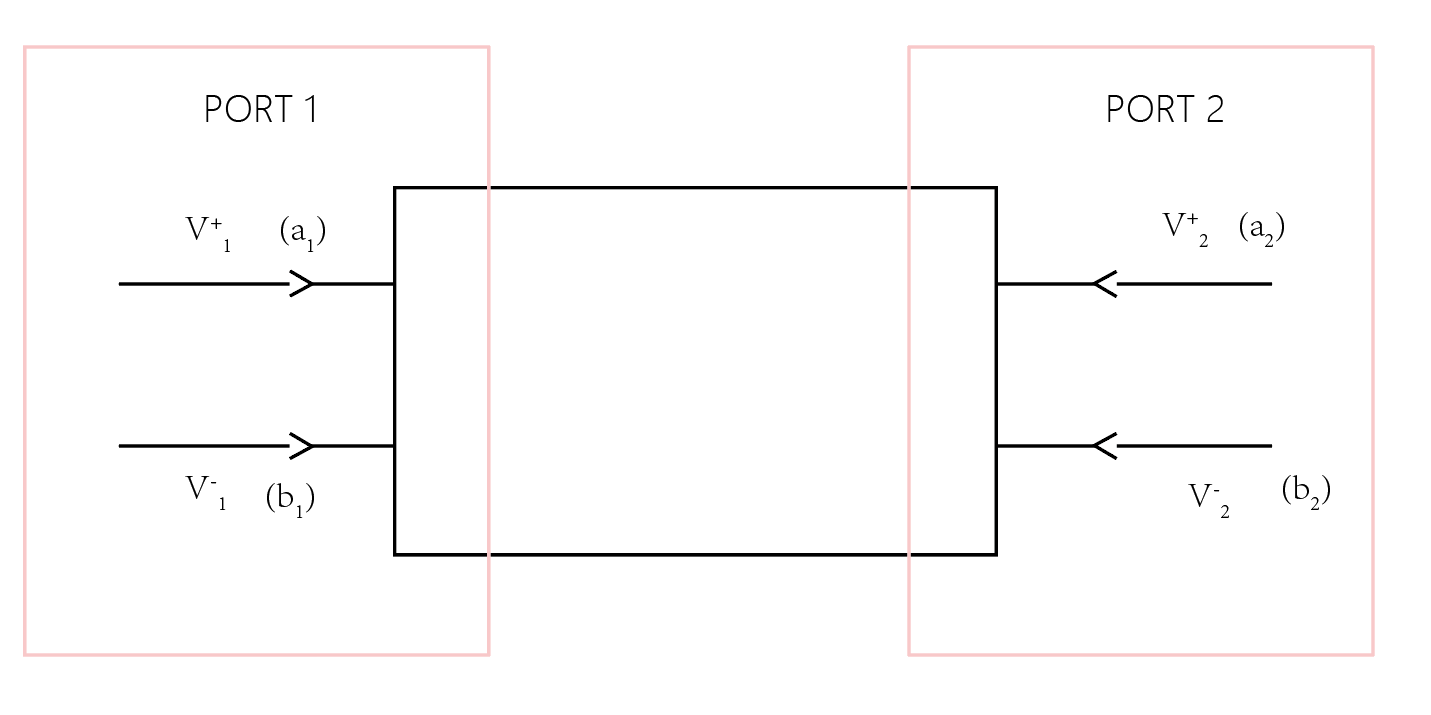
\includegraphics[width=0.7\textwidth]{two_terminal_a.png}
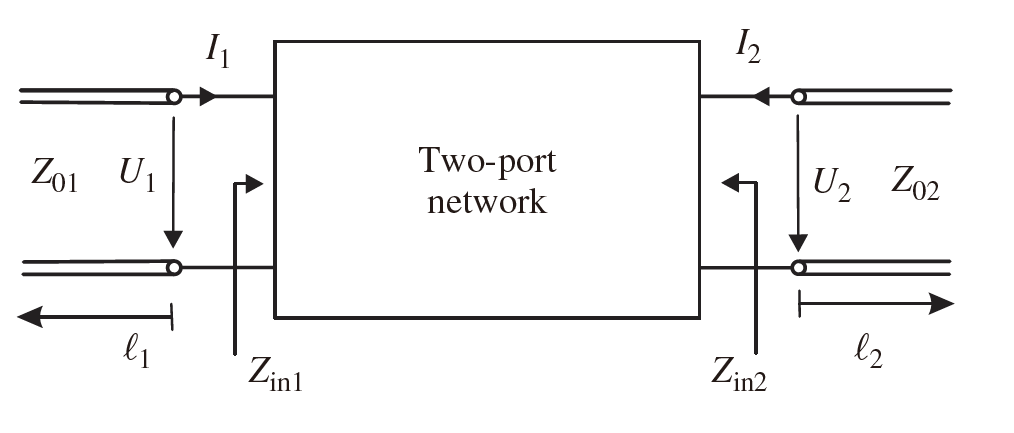
\includegraphics[width=0.7\textwidth]{two_terminal_b.png}
\caption{二端口网络}
\end{figure}
但是做题的时候是从非归一化($V_i,\; I_i$)出发, 将其用归一化来表示($v_i=a_i+b_i,\; i_i=a_i-b_i$), 则可以得到
\begin{align}
  V_i&=\sqrt{Z_{0_i}}\cdot (a_i+b_i)
  \\I_i&=\frac{a_i-b_i}{\sqrt{Z_{0_i}}}
\end{align}
将式子整理成为用$b_i$来表示$a_i$的形式, 可以利用克莱姆法则来求解. 
\begin{equation}
  \begin{cases}
    ax+by=e
    \\ cx+dy=f
  \end{cases}
\end{equation}
可以得到
\begin{gather}
  x=\frac{\begin{vmatrix}
    e&b
    \\ f&d
  \end{vmatrix}}{\begin{vmatrix}
    a&b
    \\ c&d
  \end{vmatrix}}
\end{gather}
\begin{gather}
  y=\frac{\begin{vmatrix}
    a&e
    \\ c&f
  \end{vmatrix}}{\begin{vmatrix}
    a&b
    \\ c&d
  \end{vmatrix}}
\end{gather}
将含有$a_1,\; a_2$的项移到方程组右端, 作为$e,\; f$. 而$b_1,\; b_2$的系数则分别为$a,\; b, \; c, \; d$

通常会设$r=\frac{Z_{C2}}{Z_{C1}}=\frac{Y_{C1}}{Y_{C2}}$, $z=\frac{Z}{Z_{C1}}$, $y=\frac{Y}{Y_{C1}}$

再根据$[s]$参数定义易知
\begin{align*}
  s_{11}=\frac{b_1}{a_1}\mid_{a_2=0}
  \\  s_{12}=\frac{b_1}{a_2}\mid_{a_1=0}
  \\  s_{21}=\frac{b_2}{a_1}\mid_{a_2=0}
  \\  s_{22}=\frac{b_2}{a_2}\mid_{a_1=0}
\end{align*}
来求出各个参数. 
\subsection{偶模奇模求法}
当二端口网络两边的特征阻抗相等且对称时可以使用本方法

Even and odd modes are the two main modes of propagation of the signal through a coupled transmission line pair. 

对于对称二端口网络, 满足
\begin{equation}
  \begin{cases}
    s_{11}=s_{22}
    \\ s_{12}=s_{21}
  \end{cases}
\end{equation}
则其S参数矩阵可以写成
\begin{equation}
  [s]=\begin{bmatrix}
    s_{11}&s_{21}
    \\ s_{21}&s_{11}
  \end{bmatrix}
\end{equation}
现在的问题在于$s_{11}$和$s_{21}$如何求得. 我们可以使用本征值来表示$s_{11}$和$s_{21}$. 
\begin{equation}
  \begin{cases}
    s_{11}=\frac{s_1+s_2}{2}
    \\ s_{21}=\frac{s_1-s_2}{2}
  \end{cases}
\end{equation}
本征值$s_1$和$s_2$可以分别由开路同相激励和短路反向激励求得

将电路以中间为分割线对称分割, 注意如果中间串联一个阻抗为$Z$的元件将其拆成$\frac{Z}{2}$, 并联一个导纳为$Y$的元件将其拆成$\frac{Y}{2}$
通常会隐含着$Z=\frac{1}{Y}$的条件
\subsubsection{同相偶模激励}
对称面为磁壁, 相当于\textbf{开路}

分割段直接整开路, 然后就变成传输线与终端负载的情况, 此时的反射系数$\Gamma$就是本征值$s_1$
$$s_1=\Gamma_{\text{open}}=\frac{Z_L-Z_C}{Z_L+Z_C}$$
若负载用$Y$表示则统一化为$Z$
\subsubsection{反相奇模激励}
对称面为电壁, 相当于\textbf{短路}

分割段直接整短路, 然后就变成传输线与终端负载的情况, 此时的反射系数$\Gamma$就是另一个本征值$s_2$
$$s_2=\Gamma_{\text{short}}=\frac{Z_L-Z_C}{Z_L+Z_C}$$
若负载用$Y$表示则统一化为$Z$

\section{ABCD矩阵}
The ABCD-parameters are known variously as chain, cascade, or transmission parameters.

用于网络级联, 使用电压电流来定义. 

二端口网络的ABCD参数可以写成
\begin{align*}
  V_1&=A\cdot V_2+B\cdot I_2
  \\ I_1&=C\cdot V_2+D\cdot I_2
\end{align*}
或者写成矩阵
\[
  \begin{bmatrix}
    V_1\\
    I_1
  \end{bmatrix}
  =
  \begin{bmatrix}
    A&B\\
    C&D
  \end{bmatrix}
  \cdot
  \begin{bmatrix}
    V_2\\
    I_2
  \end{bmatrix}
\]
\subsection{Normalized}
当然也可以使用归一化表示
\[
  \begin{bmatrix}
    v_1\\
    i_1
  \end{bmatrix}
  =
  \begin{bmatrix}
    \bar{a}&\bar{b}\\
    \bar{c}&\bar{d}
  \end{bmatrix}
  \cdot
  \begin{bmatrix}
    v_2\\
    i_2
  \end{bmatrix}
\]
归一化电压$v_i=a_i+b_i=\frac{V_i}{\sqrt{Z_{0_i}}}$, 归一化电流$i_i=a_i-b_i=\sqrt{Z_{0_i}}\cdot I_i$
% 但是做题的时候是从非归一化($V_i,\; I_i$)出发, 将其用归一化来表示($v_i=a_i+b_i,\; i_i=a_i-b_i$), 则可以得到
% \begin{align*}
%   V_i&=\sqrt{Z_{0_i}}\cdot (a_i+b_i)
%   \\I_i&=\frac{a_i-b_i}{\sqrt{Z_{0_i}}}
% \end{align*}


\section{散射传输参数}
Scattering transfer parameters (T-parameters)

与ABCD参数不同, T参数使用入射波$a_i$和反射波$b_i$来定义(已经归一化了)

\textbf{注意}$a,\; b$\textbf{的顺序是反的, 和其他参数不一样. }
\[
  \begin{bmatrix}
    a_1\\
    b_1
  \end{bmatrix}
  =
  \begin{bmatrix}
    t_{11}&t_{12}\\
    t_{21}&t_{22}
  \end{bmatrix}
  \cdot
  \begin{bmatrix}
    b_2\\
    a_2
  \end{bmatrix}
\]


\section{信号流图}
每个节点为$a_i$和$b_j$, 箭头上面\footnote{S参数第一个角标为输出(反射波), 第二个角标为输入(入射波)}则是$s_{ji}$
\begin{itemize}
  \item 串联法则 头尾相同的线, 上边增益的加起来
  \item 并联法则 头尾相接的线, 中间的节点去掉然后相乘
  \item 自闭环(Self-Loop)法则 
\end{itemize}

\section{参数转换}

\subsection{S parameter and Z parameter}
S to Z
\begin{align*}
  z_{11}=\frac{1+s_{11}-s_{22}-\det(s)}{1-s_{11}-s_{22}+\det(s)}
  \\ z_{12}=\frac{2\cdot s_{12}}{1-s_{11}-s_{22}+\det(s)}
  \\ z_{21}=\frac{2\cdot s_{21}}{1-s_{11}-s_{22}+\det(s)}
  \\ z_{22}=\frac{1-s_{11}+s_{22}-\det(s)}{1-s_{11}-s_{22}+\det(s)}
\end{align*}
或者写成矩阵形式
\begin{equation}
  [z]=(I_n-[s])^{-1}\times (I_n+[s])
\end{equation}
\subsection{S parameter and T parameter}
S to T
\begin{equation}
  [t]=\frac{1}{s_{21}}\begin{bmatrix}
    1&-s_{22}
    \\ s_{11}&\det(\textbf{s})
  \end{bmatrix}
\end{equation}
T to S
\begin{equation}
  [s]=\frac{1}{t_{11}}\cdot\begin{bmatrix}
    t_{21}&\det(\textbf{t})
    \\ 1 & -t_{12}
  \end{bmatrix}
\end{equation}

\chapter{无源微波网络}
\section{断路器}
不吸收入射波的任何能量而使其产生全反射。实用的短路器都作成可调的,称为可调短路活塞。
\section{衰减器}
\subsection{截止式衰减器}
\begin{equation}
  [s]=\begin{bmatrix}
    0& e^{\alpha\cdot l}
    \\ e^{\alpha\cdot l}&0
  \end{bmatrix}
\end{equation}
衰减系数$$\alpha\approx\frac{2\pi}{\lambda_c}\quad \lambda\gg\lambda_c$$
起衰减作用的是圆波导, 其工作模式是$TE_{11}$模. 
衰减器的衰减量为(单位为dB)
$$L(l)=L(0)+8.68\cdot\alpha\cdot l$$
% \section{截止式衰减器}
\subsection{旋转极化式衰减器}
\begin{equation}
  [s]=\begin{bmatrix}
    0&\cos^2{\theta}
    \\ \cos^2{\theta}&0
  \end{bmatrix}
\end{equation}

% 功率分配器和定向耦合器, 对应无源微波网络一章. 
\section{三端口网络(T型结)}
Power Dividers 最简单的就是T型结. 它是有一个输入和两个输入(或者两个输入一个输出)的三端口网络. 
任意三端口网络都有九个独立的矩阵元. 

若所有端口都是匹配的, 则有$S_ii=0$(对角线为0)
\begin{gather}
  [S]=\begin{bmatrix}
    0&S_{12}&S_{13}
    \\ S_{21}&0&S_{23}
    \\ S_{31}&S_{32}&0
  \end{bmatrix}
\end{gather}
若网络是互易(Reciprocal)的, $S_{ij}=S_{ji}$, 以下统一为$S_{ij}$表示. 
\begin{gather}
  [S]=\begin{bmatrix}
    0&S_{12}&S_{13}
    \\ S_{12}&0&S_{23}
    \\ S_{13}&S_{23}&0
  \end{bmatrix}
\end{gather}
若网络是无耗(Lossless)的, 则满足Unitary条件(\ref{eq:unitary}). 即
\begin{quotation}
  $[S]$的任一列与此列的共轭点乘等于1. $[S]$的任一列与不同列的共轭点乘等于0. 
\end{quotation}
可以列出
\begin{equation}
  \begin{cases}
    \lvert S_{12}\rvert ^2+\lvert S_{13}\rvert ^2=1 &\text{即}c_1\cdot c_1^H
    \\ \lvert S_{12}\rvert ^2+\lvert S_{23}\rvert ^2=1 &\text{即}c_2\cdot c_2^H
    \\ \lvert S_{13}\rvert ^2+\lvert S_{23}\rvert ^2=1 &\text{即}c_3\cdot c_3^H
  \end{cases}
    \label{eq:t_junction_unitary_1}
\end{equation}
\begin{equation}
  \begin{cases}
    0\cdot S_{12}^H+S_{12}\cdot 0+S_{13}\cdot S_{23}^H=0 &\text{即}c_1\cdot c_2^H
    \\ 0\cdot S_{13}^H+S_{12}\cdot S_{23}^H+S_{13}\cdot 0=0 &\text{即}c_1\cdot c_3^H
    \\ S_{12}\cdot S_{13}^H+0\cdot S_{23}^H+S_{23}\cdot 0=0 &\text{即}c_2\cdot c_3^H
  \end{cases}
\end{equation}
化简可得
\begin{equation}
  \begin{cases}
    S_{13}\cdot S_{23}^H=0
    \\ S_{12}\cdot S_{23}^H=0
    \\ S_{12}\cdot S_{13}^H=0
  \end{cases}
  \label{eq:t_junction_unitary_2}
\end{equation}
但\ref{eq:t_junction_unitary_2}总和\ref{eq:t_junction_unitary_1}矛盾, 这就表明了三端口网络不可能同时是无耗的, 互易的和全部端口匹配的. 

\begin{itemize}
  \item 无耗, 互易三端口网络不能同时匹配, 即$S_{ii}$不可能全为零
  \item 无耗互易的两个端口不可能同时实现匹配, 否则退化为二端口网络
  \item 端口全匹配, 无耗非互易三端口网络是理想环形器
\end{itemize}

对于$E-T$分支有以下性质, 高的竖着的, 上边的是PORT 3. 
\begin{itemize}
  \item 1, 2等幅反相输出 $s_{13}= -s_{23}$ ,功率均分(3dB)
  \item 1, 2等幅反相激励,3有输出,功率合成
  \item 1, 2等幅同相激励,3无输出
\end{itemize}
对于$H-T$分支有以下性质, 平的的躺着的, 躺着对过去没东西的是PORT 3. 
\begin{itemize}
  \item 1, 2等幅同相输出 $s_{13}= s_{23}$ ,功率均分(3dB)
  \item 1, 2等幅同相激励,3有输出,功率合成
  \item 1, 2等幅反相激励,3无输出
\end{itemize}
% \subsection{非互易但全匹配且无耗}
% 环形器(circulator)
% \subsection{仅两个匹配但互易且无耗}
% \subsection{非无耗(有损)但互易且全匹配}
% 电阻性功率分配器
\section{定向耦合器}
由互易且全匹配可以得到
\begin{equation}
  [S]=\begin{bmatrix}
    0&S_{12}&S_{13}&S_{14}
    \\S_{12}&0&S_{23}&S_{24}
    \\S_{13}&S_{23}&0&S_{34}
    \\S_{14}&S_{24}&S_{34}&0
  \end{bmatrix}
\end{equation}
设PORT 1, 4隔离, 得到$s_{14}=s_{41}=s_{32}=s_{32}=0$ 

设$s_{12}=\alpha,\; s_{13}=j\beta$利用Unitary条件可以得到
\begin{equation}
  [s]=\begin{bmatrix}
    0&\alpha&j\beta&0
    \\ \alpha &0&0&j\beta
    \\ j\beta &0&0&\alpha
    \\ 0 &j\beta &\alpha &0
  \end{bmatrix}
\end{equation}


\section{波导双T和Magic T}
\subsection{波导双T}
\begin{figure}[H]
\centering
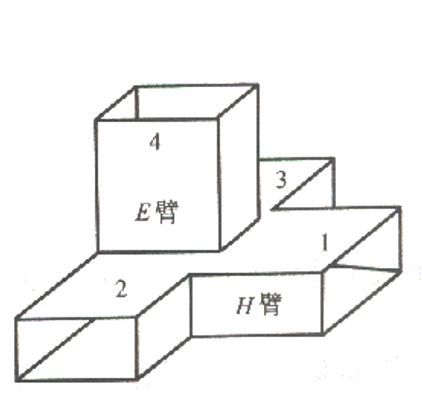
\includegraphics[width=0.33\textwidth]{double_t.png}
\caption{波导双T}
\end{figure}
\begin{itemize}
  \item 4(E臂)输入,2, 3等幅反相输出 $s_{24}= -s_{34} $,功率均分(3dB)
  \item 1(H臂)输入,2, 3等幅同相输出 $s_{31}= s_{21} $,功率均分(3dB)
  \item 1, 4端口(H臂和E臂)相互隔离$s_{41}=s_{14}=0$
  \item 对称和互易
\end{itemize}
\subsection{Magic T}
魔T的S参数矩阵为 (1端口为H臂, 4端口为E臂)
\begin{equation}
  [s]=\frac{1}{\sqrt{2}}\cdot\begin{bmatrix}
    0&1&1&0
    \\ 1&0&0&1
    \\ 1&0&0&-1
    \\ 0&1&-1&0
  \end{bmatrix}
\end{equation}
性质
\begin{itemize}
  \item 1, 4端口(H臂和E臂)匹配, 2, 3端口也会自动达到匹配
  \item 1, 4端口(H臂和E臂)隔离, 2, 3端口也会相互隔离
\end{itemize}
\begin{align*}
  [a]=[\hat{a}]+[\Gamma] [b]
  \\ [b]=[s] [a]
\end{align*}
% $[\hat{a}]$表示信号源输入(一般是从H臂\footnote{端口1}输入), 
若信号由H臂\footnote{端口1}输入为$\hat{a_1}$, 端口2, 3的反射系数分别为$\Gamma_2,\; \Gamma_3$. 则$[a]$就为
\begin{gather}
  [a]=[\hat{a}]+[\Gamma] [b]=\begin{bmatrix}
    \hat{a_1}\\
    \Gamma_2 \cdot b_2
    \\ \Gamma_3 \cdot b_3
    \\ 0
  \end{bmatrix}
\end{gather}
就可以根据$[b]=[s][a]$求出相应的各端口的反射波


\chapter{Microwave Resonators}
\section{矩形谐振腔}
$TE_{mnp}$谐振模式的波数$k$
\begin{align*}
  k=\sqrt{(\frac{m\pi}{a})^2+(\frac{n\pi}{b})^2+(\frac{p\pi}{l})^2}
\end{align*}
谐振频率$f_0$
$$f_0=\frac{c}{2\pi}\cdot k$$
\section{圆柱腔}
\subsection{TE mode}
$TE_{nip}$ mode, 表会给出$v_{ni}$
$$k=\sqrt{(\frac{v_{ni}}{a})^2+(\frac{p\pi}{l})^2}$$
\subsection{TM mode}
$TM_{nip}$ mode, 表会给出$u_{ni}$
$$k=\sqrt{(\frac{u_{ni}}{a})^2+(\frac{p\pi}{l})^2}$$

\end{document}